
\documentclass[11pt, a4paper]{article}
%\usepackage{proj1}
\usepackage{natbib}
\usepackage{fancyhdr}  
\usepackage{subcaption}
\usepackage{caption}
\usepackage{graphicx}
\usepackage{numprint}
\usepackage{multirow}
\linespread{1.25} 
\setlength{\parindent}{0cm}
\graphicspath{{Images/}}
\usepackage{hyperref}
\usepackage{amsmath}
\usepackage{amsfonts}
\usepackage{amssymb}
\usepackage{amsthm}
\usepackage{mathtools}
\usepackage{commath}
\usepackage{bbm}

%\usepackage[sc,osf]{mathpazo}
\usepackage{subcaption}
\usepackage[a4paper, top=1in, left=1.0in, right=1.0in, bottom=1in, includehead, includefoot]{geometry} %Usually have top as 1in

\usepackage{listings}
\usepackage{color} %red, green, blue, yellow, cyan, magenta, black, white
\definecolor{mygreen}{RGB}{28,172,0} % color values Red, Green, Blue
\definecolor{mylilas}{RGB}{170,55,241}


\hypersetup{colorlinks,linkcolor={black},citecolor={blue},urlcolor={black}}
\usepackage{color}
\urlstyle{same}


\theoremstyle{definition}
\newtheorem{definition}{Definition}[section]

\newcommand{\adja}{q_a}
\newcommand{\adjb}{q_b}
\newcommand{\adjaB}{q_{a,\partial \Omega}}
\newcommand{\adjbB}{q_{b,\partial \Omega}}
\newcommand{\adjB}{q_{\partial \Omega}}
\newcommand{\Adja}{\mathbf{p}}
\newcommand{\Adjb}{q}
\newcommand{\adj}{q}
\newcommand{\Adjc}{{q}_{\partial \Omega}}
\newcommand{\ra}{\rho_a}
\newcommand{\rb}{\rho_b}
\newcommand{\w}{\mathbf{w}}
\newcommand{\x}{\mathbf{x}}
\newcommand{\f}{\mathbf{f}}
\newcommand{\ve}{\mathbf{v}}
\newcommand{\n}{\mathbf{n}}
\newcommand{\h}{\mathbf{h}}
\newcommand{\K}{\mathbf{K}}
\newcommand{\hr}{\widehat \rho}
\newcommand{\jf}{\mathbf j}

\DeclareMathOperator{\sgn}{sgn}
\DeclareMathOperator{\Grad}{Grad}
\DeclareMathOperator{\Div}{Div}
\DeclareMathOperator{\Lap}{Lap}
%	\begin{figure}[h]
%		\centering
%		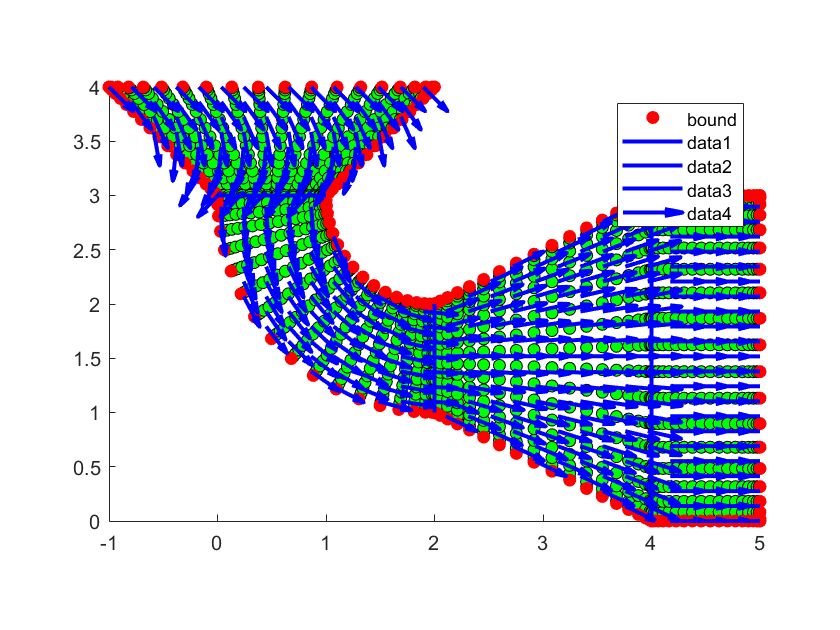
\includegraphics[scale=0.35]{F1.png}
%		\caption{Forward $\rho$ for $a = 0.01$} 
%		\label{F1}
%	\end{figure}

\begin{document}
	
\section{Newton-Krylov }

	One question I have is why the solver needs more than one iteration, if the given solution is exact.
Check that no-flux interacting is correct.\\
\\
We have the following problems, differences measured with the $L_1/L_2$ norm, with $N = 16$, and with optimality tolerance $10^{-4}$ in the old code:\\
Dirichlet exact, Error $= 2.1631 \times 10^{-16}$, time = $ 120$ s,\\
Dirichlet with $\kappa =1$, Error $= 4.8164 \times 10^{-6}$, time = $120 $ s va $480$ s,\\
Dirichlet exact with $V_{ext}$, Error $= 0.0027$, time = $ 130$ s.\\
Then for the Neumann problems we have, with $N = 20$:\\
Neumann exact, Error $= 2.3286 \times 10^{-15}$, time = $1.0824 \times 10^3 $ s,\\ I ran the original code for this, which gives $228$ s.
I think I messed with the timing of the algorithm somehow... 

(++ note: we fix the slowness by choosing to eliminate the flags. We get $4.1841 \times 10^{-9}$ for the interacting Neumann case)

\section{Hodge Helmholtz Decomposition}
We choose a basis of Lagrange polynomials (dimension $2(p-1)p$) and choose an element $v$ from this basis. 
We then note that if $v$ satisfies $\nabla \times v = 0$, we can write $Dv =0$, where $D$ is the discretized curl. Then we can split this into two parts, such that $Dv = D_1 v_1 + D_2 v_2 =0$. We determine that $(p-1)^2$ is the degree of interpolation	polynomial and furthermore, this implies that $(p -1)^2$ rows of $D$ are linearly independent. Therefore, we split up $D$ such that $D_2$ has $(p -1)^2$ rows and is invertible. We can then see that 
\begin{align*}
	v_2 = -D_2^{-1} D_1 u_1,
\end{align*}
which provides a formula for creating a vector $\mathbf v = (v_1, v_2)$ satisfying that $\nabla \times v = 0$.
We can then choose $p^2 -1$ of such vectors as a basis of the curl free vector space.
Any curl free vector field $\mathbf w$ can then be described as a linear combination of these, i.e. $\mathbf w = \sum_i \alpha_i v_i$.\\
A similar argument can be used to construct a divergence free basis. The harmonic part of the vector field is found by subtracting the curl free and divergence free parts from the original field.
\section{Curl free control}	
We consider
\begin{align*}
	&\min_{\rho, \w} \frac{1}{2}\int_0^T \int_\Omega \left(\rho - \hr\right)^2 d\x dt + \frac{\beta}{2}\int_0^T \int_\Omega \w^2 d\x dt + \frac{\eta}{2}\int_0^T \int_\Omega \left(\nabla \times \w \right)^2 d\x dt\\
	&\text{subject to:}\\
	& \frac{\partial \rho}{\partial t} = \nabla^2 \rho - \nabla \cdot \left(\rho \w\right)\\
	& \frac{\partial \rho}{\partial n} - \rho \w \cdot \n = 0
\end{align*}
We know that in two dimensions
\begin{align*}
    \nabla \times \w = \frac{\partial w_2}{\partial x_1}  - \frac{\partial w_1}{\partial x_2},
\end{align*}
and so the Lagrangian is
\begin{align*}
	\mathcal L (\rho, \w ,q_1, q_2) =& \frac{1}{2}\int_0^T \int_\Omega \left(\rho - \hr\right)^2 d\x dt + \frac{\beta}{2}\int_0^T \int_\Omega \w^2 d\x dt + \frac{\eta}{2}\int_0^T \int_\Omega \left(\frac{\partial w_2}{\partial x_1}  - \frac{\partial w_1}{\partial x_2} \right)^2 d\x dt\\
	&- \int_0^T \int_\Omega q_1 \left(\frac{\partial \rho}{\partial t} - \nabla^2 \rho + \nabla \cdot \left(\rho \w\right) \right) d \x dt \\
	&- \int_0^T \int_{\partial \Omega} q_2\left(\frac{\partial \rho}{\partial n} - \rho \w \cdot \n \right) d\x dt.
\end{align*}
Then, since we know that $q_1 = q_2$, we get
\begin{align*}
	\mathcal L (\rho, \w ,q) =& \frac{1}{2}\int_0^T \int_\Omega \left(\rho - \hr\right)^2 d\x dt + \frac{\beta}{2}\int_0^T \int_\Omega \w^2 d\x dt + \frac{\eta}{2}\int_0^T \int_\Omega \left(\frac{\partial w_2}{\partial x_1}  - \frac{\partial w_1}{\partial x_2} \right)^2 d\x dt\\
	&- \int_0^T \int_\Omega -\rho\frac{\partial q}{\partial t} - \rho \nabla^2 q - \nabla q \cdot \left(\rho \w\right) d \x dt  - \int_\Omega q(T) \rho(T) - q(0) \rho(0) d\x\\
	&- \int_0^T \int_{\partial \Omega}  - \rho \nabla q \cdot \n  d\x dt.
\end{align*}
For the adjoint equation, we find the usual results.
We take the derivative with respect to $\w$
\begin{align*}
	\mathcal L_\w(\rho, \w, q)h &= \int_0^T \int_\Omega \beta \w \cdot  \h + \rho \nabla q \cdot \h + \eta \left(\frac{\partial w_2}{\partial x_1} \frac{\partial h_2}{\partial x_1} - \frac{\partial w_2}{\partial x_1}\frac{\partial h_1}{\partial x_2} - \frac{\partial h_2}{\partial x_1}\frac{\partial w_1}{\partial x_2} +  \frac{\partial w_1}{\partial x_2}\frac{\partial h_1}{\partial x_2}\right) d\x dt.
\end{align*}
Collecting terms in $h_1$ and $h_2$ we get
\begin{align*}
	\mathcal L_\w(\rho, \w, q)h =& \int_0^T \int_\Omega 
	h_1 \left( \beta w_1 + \rho \frac{\partial q}{\partial x_1} \right)+
	h_2 \left( \beta w_2 + \rho \frac{\partial q}{\partial x_2} \right)\\
    &+\frac{\partial h_1}{\partial x_2} \eta \left(- \frac{\partial w_2}{\partial x_1} + \frac{\partial w_1}{\partial x_2}\right)+
	\frac{\partial h_2}{\partial x_1} \eta \left(\frac{\partial w_2}{\partial x_1} -\frac{\partial w_1}{\partial x_2} \right)
	d\x dt\\
	=& \int_0^T \int_\Omega 
	h_1 \left( \beta w_1 + \rho \frac{\partial q}{\partial x_1} \right)+
	h_2 \left( \beta w_2 + \rho \frac{\partial q}{\partial x_2} \right)\\
	&- h_1 \eta \left(- \frac{\partial^2 w_2}{\partial x_1 x_2} + \frac{\partial^2 w_1}{\partial x_2^2}\right)
	- h_2 \eta \left(\frac{\partial^2 w_2}{\partial x_1^2} -\frac{\partial^2 w_1}{\partial x_1x_2} \right) d \x dt\\
	&+ \int_0^T \int_{\partial \Omega} h_1 \eta \left(- \frac{\partial w_2}{\partial n_1} + \frac{\partial w_1}{\partial n_2} \right) + h_2 \eta \left(\frac{\partial w_2}{\partial n_1} -\frac{\partial w_1}{\partial n_2} \right)
	d\x dt.
\end{align*}
Then
\begin{align*}
	\mathcal L_\w(\rho, \w, q)h =&  \int_0^T \int_\Omega \h \left(\beta \w + \rho \nabla q\right) + \eta \h \left(\frac{\partial^2 w_2}{\partial x_1 x_2}, \frac{\partial^2 w_1}{\partial x_1x_2}   \right) - \eta \h \left(\frac{\partial^2 w_1}{\partial x_2^2},\frac{\partial^2 w_2}{\partial x_1^2} \right) d\x dt\\
	&+ \int_0^T \int_{\partial \Omega} \eta \h \left(-\frac{\partial w_2}{\partial n_1} +\frac{\partial w_1}{\partial n_2}, \frac{\partial w_2}{\partial n_1} -\frac{\partial w_1}{\partial n_2} \right) d\x dt
\end{align*}
So we can extract
\begin{align*}
	\beta \w + \rho \nabla q + \eta \left(\frac{\partial^2 w_2}{\partial x_1 x_2} -\frac{\partial^2 w_1}{\partial x_2^2} , \frac{\partial^2 w_1}{\partial x_1x_2} -\frac{\partial^2 w_2}{\partial x_1^2}  \right) &= 0 \quad \text{in} \quad \Omega\\
	\eta \left(-\frac{\partial w_2}{\partial n_1} +\frac{\partial w_1}{\partial n_2}, \frac{\partial w_2}{\partial n_1} -\frac{\partial w_1}{\partial n_2} \right) &= 0 \quad \text{on} \quad \partial \Omega
\end{align*}
The first components give
\begin{align*}
	&\beta w_1 - \eta \frac{\partial^2 w_1}{\partial x_2^2} = \rho \frac{\partial q}{\partial x_1} - \eta\frac{\partial^2 w_2}{\partial x_1 x_2} \quad \text{in} \quad \Omega\\
	&\eta\left( -\frac{\partial w_2}{\partial n_1} +\frac{\partial w_1}{\partial n_2} \right) = 0 \quad \text{on} \quad \partial \Omega
\end{align*}
and the second are
\begin{align*}
	&\beta w_2 - \eta \frac{\partial^2 w_2}{\partial x_1^2} = \rho \frac{\partial q}{\partial x_2} - \eta \frac{\partial^2 w_1}{\partial x_1x_2}\quad \text{in} \quad \Omega\\
	&\eta \left(\frac{\partial w_2}{\partial n_1} -\frac{\partial w_1}{\partial n_2} \right) = 0 \quad \text{on} \quad \partial \Omega.
\end{align*}










\end{document}